\section{Experimental results}

In both of our experiments, a toy query, "usa election president politics " was used. We first tried 
only TF-IDF and then a combined retrieval with rankType = TODO, both of which were compared to combined 
retrieval with rankType = TODO. We graded the top ten results of each retrieval as relevant or not and 
plotted a precision vs recall graph for each of them.

\subsection{TF-IDF only}

\begin{figure}[H]
\centering
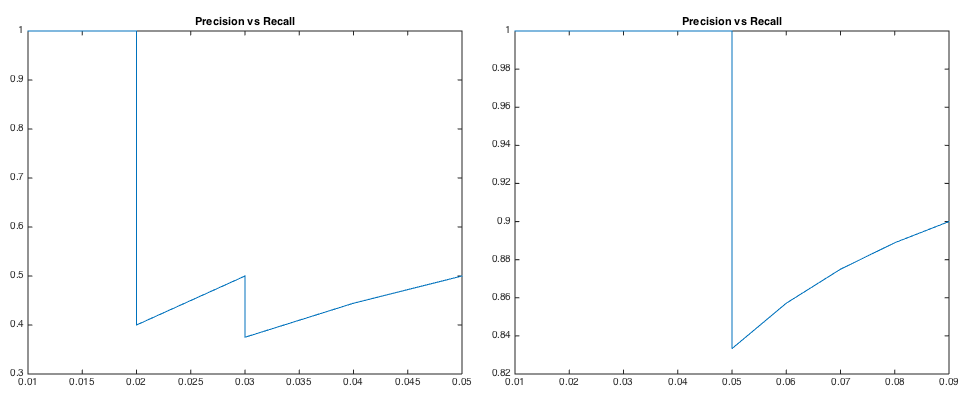
\includegraphics[width=5.5in,natwidth=534,natheight=345]{images/exptfidf.png}
\caption{Precision vs Recall for TF-IDF only (left) and combination with $\alpha = 0.5$ and rankType = TODO (right).}
\label{fig:exptfidf}
\end{figure}

As expected, a combination of TF-IDF with PageRank performs better than just the first algorithm.
The problem is that our database does not contain \emph{all} the tweets of each user, so the bag
of words model is only precise among the crawled topics. If, for instance, a user posts a single tweet
about politics and we only crawl that tweet for that user, it's going to appear really well-ranked for
TF-IDF while, in reality, it shouldn't. When PageRank is added to the equation we exploit the
graph structure of Twitter and take the authority of the aforementioned user in consideration, which
highly improves our Precision vs Recall curve, as can be seen in Figure \ref{fig:exptfidf}.

\subsection{PageRank variant}

\subsection{Evaluation}
Summary of what alpha should be and why.
